\documentclass[11pt,table]{beamer}
\mode<presentation>
\usepackage{etex}
\usepackage{graphicx}
\usepackage{epstopdf}
\usepackage[english]{babel}
\usepackage{tabularx}
\usepackage{booktabs}
\usepackage{mathrsfs}
\usepackage{multicol}
\usepackage{bm}
\usepackage{subcaption}
\usepackage{wrapfig}
\usepackage{dcolumn}
\usepackage{threeparttable}
\usepackage{booktabs}
\usepackage{bbm}
\usepackage{amsmath,dsfont,listings}
\usepackage{amssymb}
\usepackage{rotating}
\usepackage{multirow}
\usepackage{tcolorbox}
\usepackage[authoryear]{natbib}
\usepackage{circledsteps}
\usepackage{qtree}

\usepackage{tikz}
\usetikzlibrary{arrows,decorations.pathmorphing,backgrounds,fit,positioning,shapes.symbols,chains}
\setbeamertemplate{section in toc}[sections numbered]
\setbeamertemplate{caption}[numbered]

\bibliographystyle{Econometrica}

\setbeamersize{text margin right=3.5mm, text margin left=7.5mm}  % text margin
\setbeamersize{sidebar width left=0cm, sidebar width right=0mm}
\setbeamertemplate{sidebar right}{}
\setbeamertemplate{sidebar left}{}

\definecolor{text-grey}{rgb}{0.45, 0.45, 0.45} % grey text on white background
\definecolor{bg-grey}{rgb}{0.66, 0.65, 0.60} % grey background (for white text)
\definecolor{fu-blue}{RGB}{0, 51, 102} % blue text
\definecolor{fu-green}{RGB}{153, 204, 0} % green text
\definecolor{fu-red}{RGB}{204, 0, 0} % red text (used by \alert)
\definecolor{BrewerBlue}{HTML}{377EB8} % Define Brewer Blue
\definecolor{BrewerRed}{HTML}{E41A1C}  % Define Brewer Red

\setbeamertemplate{frametitle}{%
    \vskip-30pt \color{text-grey}\large%
    \begin{minipage}[b][23pt]{\textwidth}%
    \flushleft\insertframetitle%
    \end{minipage}%
}

\setbeamertemplate{navigation symbols}{} 

%%% begin title page
\setbeamertemplate{title page}{
\vskip2pt\hfill
\vskip19pt\hskip3pt

% set the title and the author
\vskip4pt
\parbox[top][1.35cm][c]{11cm}{\LARGE\color{text-grey} \textcolor{red1}{RL}earning:\\[1ex] \inserttitle \\[1ex] \small \quad \\[3ex]}
\vskip17pt
\parbox[top][1.35cm][c]{11cm}{\small Unit 1-4: \insertsubtitle \\[2ex] \insertauthor \\[1ex]}
}
%%% end title page

%%% colors
\usecolortheme{lily}
\setbeamercolor*{normal text}{fg=black,bg=white}
\setbeamercolor*{alerted text}{fg=fu-red}
\setbeamercolor*{example text}{fg=fu-green}
\setbeamercolor*{structure}{fg=fu-blue}

\setbeamercolor*{block title}{fg=white,bg=black!50}
\setbeamercolor*{block title alerted}{fg=white,bg=black!50}
\setbeamercolor*{block title example}{fg=white,bg=black!50}

\setbeamercolor*{block body}{bg=black!10}
\setbeamercolor*{block body alerted}{bg=black!10}
\setbeamercolor*{block body example}{bg=black!10}

\setbeamercolor{bibliography entry author}{fg=fu-blue}
\setbeamercolor{bibliography entry journal}{fg=text-grey}
\setbeamercolor{item}{fg=fu-blue}
\setbeamercolor{navigation symbols}{fg=text-grey,bg=bg-grey}
%%% end colors

%%% headline
\setbeamertemplate{headline}{
\vskip30pt
}
%%% end headline

%%% footline
\newcommand{\footlinetext}{
%\insertshortinstitute, \insertshorttitle, \insertshortdate
}
\setbeamertemplate{footline}{
\vskip2pt
\hfill \raisebox{-1pt}{\usebeamertemplate***{navigation symbols}}
\hfill \insertframenumber\hspace{10pt}
\vskip4pt
}
%%% end footline

%%% settings for listings package
\lstset{extendedchars=true, showstringspaces=false, basicstyle=\footnotesize\sffamily, tabsize=2, breaklines=true, breakindent=10pt, frame=l, columns=fullflexible}
\lstset{language=Java} % this sets the syntax highlighting
\lstset{mathescape=true} % this switches on $...$ substitution in code
% enables UTF-8 in source code:
\lstset{literate={ä}{{\"a}}1 {ö}{{\"o}}1 {ü}{{\"u}}1 {Ä}{{\"A}}1 {Ö}{{\"O}}1 {Ü}{{\"U}}1 {ß}{\ss}1}
%%% end listings

\usepackage{concmath}
\usepackage{xcolor}
\definecolor{red1}{RGB}{206, 17, 38}
\definecolor{blue1}{RGB}{16, 118, 208}
\definecolor{gray1}{RGB}{117, 115, 115}
\usepackage{hyperref}


\newtheorem{proposition}{Proposition}
\newtheorem{assumption}{Definition}

\title[]{Short guides to reinforcement learning}
\subtitle[]{Thompson Sampling}
\author[D. Rostam-Afschar]{\textcolor{gray1}{Davud Rostam-Afschar (Uni Mannheim)}}
\date[]{\today}
\subject{Econometrics}
\renewcommand{\footlinetext}{\insertshortinstitute, \insertshorttitle, \insertshortdate}
\hypersetup{
    bookmarks=false,
    unicode=false,
    pdftoolbar=false,
    pdffitwindow=true,
    pdftitle={Reinforcement Learning for Business, Economics, and Social Sciences: \insertsubtitle},
    pdfauthor={Davud Rostam-Afschar},
    pdfsubject={Reinforcement Learning},
    pdfkeywords={reinforcement learning, Thompson Sampling},
    pdfnewwindow=true,
}
\def\sym#1{\ifmmode^{#1}\else\(^{#1}\)\fi}

\begin{document}

\begin{frame}[plain]
  \titlepage
\end{frame}

% --------------------------------------------------- Slide --
%\begin{frame}
	%\frametitle{Content}
	%\tableofcontents[]
%\end{frame}

\section{Thompson Sampling}
{
\setbeamercolor{background canvas}{bg=BrewerBlue}
\begin{frame}
\centering
\Huge
\textcolor{white}{How to update your priors about rewards?}
\thispagestyle{empty}
\end{frame}
}





\begin{frame}{Thompson Sampling}


    \begin{itemize}
        \item Notation:

\begin{itemize}
     

\item $r^{a}_t=r_t|A_t=a$ random variable for $a$'s rewards
\item $R(a)=q(a)=\mathbb{E}\left[r^{a}_t\right]$ unknown average reward 
    \end{itemize}



        \item Idea:
\begin{itemize}
    \item  Sample several potential average rewards:


\textcolor{red1}{$R_{1}(a), \ldots, R_{d}(a) \sim \mathbb{P}\left(R(a) \mid r_{1}^{a}, \ldots, r_{t}^{a}\right)$} for each $a$


\item  Sample empirical average


$$
\textcolor{red1}{\hat{R}(a)=\frac{1}{d} \sum_{i=1}^{d} R_{i}(a)}
$$


\item  Execute \textcolor{red1}{$\underset{\operatorname{argmax}}{a} \hat{R}(a)$}


\item  Coin example


\item $\mathbb{P}\left(R(a) \mid r_{1}^{a}, \ldots, r_{t}^{a}\right)=\operatorname{Beta}\left(\theta_{a} ; \alpha_{a}, \beta_{a}\right)$


where $\alpha_{a}-1=$ \#heads and $\beta_{a}-1=\#$ tails 
\end{itemize} 
    \end{itemize}
\end{frame}





\section{Bayesian Learning}
{
\setbeamercolor{background canvas}{bg=BrewerBlue}
\begin{frame}
\centering
\Huge
\textcolor{white}{Bayesian Learning}
\thispagestyle{empty}
\end{frame}
}


\begin{frame}{Bayesian Learning}


    \begin{itemize}
        \item Notation:

\begin{itemize}
     

	\item  $\mathbb{P}\left(r^{a} ; \theta\right)$: unknown distribution (parameterized by $\theta$)

    \end{itemize}

    \item Idea:
    \begin{itemize}
        \item Express uncertainty about $\theta$ by a prior $\mathbb{P}(\theta)$
\item  Compute posterior $\mathbb{P}\left(\theta\mid r_{1}^{a}, r_{2}^{a}, \ldots, r_{t}^{a}\right)$ based on
\item  Samples $r_{1}^{a}, r_{2}^{a}, \ldots, r_{t}^{a}$ observed for $a$ so far
    \end{itemize}

    \item \textcolor{red1}{Bayes theorem:}
$$\textcolor{red1}{\mathbb{P}\left(\theta \mid r_{1}^{a}, r_{2}^{a}, \ldots, r_{t}^{a}\right) \propto \mathbb{P}\left(\theta\right) \mathbb{P}\left(r_{1}^{a}, r_{2}^{a}, \ldots, r_{t}^{a} \mid \theta\right)}$$ 
    \end{itemize}
\end{frame}

\begin{frame}{Distributional Information}


    \begin{itemize}
        \item Posterior over $\theta$ allows us to estimate

        \begin{itemize}
            \item  Distribution over next reward $r^{a}$
$$
\mathbb{P}\left(r^{a} \mid r_{1}^{a}, r_{2}^{a}, \ldots, r_{t}^{a}\right)=\int_{\theta} \mathbb{P}\left(r^{a} ; \theta\right) \mathbb{P}\left(\theta \mid r_{1}^{a}, r_{2}^{a}, \ldots, r_{t}^{a}\right) d \theta
$$
\item  Distribution over $R(a)$ when $\theta$ includes the mean

$$
\mathbb{P}\left(R(a) \mid r_{1}^{a}, r_{2}^{a}, \ldots, r_{t}^{a}\right)=\mathbb{P}\left(\theta \mid r_{1}^{a}, r_{2}^{a}, \ldots, r_{t}^{a}\right) \text { if } \theta=R(a)
$$
        \end{itemize}

        \item To guide exploration:

 \begin{itemize}
     \item UCB: \textcolor{red1}{$\mathbb{P}\left(R(a) > \operatorname{bound}\left(r_{1}^{a}, r_{2}^{a}, \ldots, r_{t}^{a}\right)\right) \geq p$}
\item  Bayesian techniques: \textcolor{red1}{$\mathbb{P}\left(R(a) \mid r_{1}^{a}, r_{2}^{a}, \ldots, r_{t}^{a}\right)$}
 \end{itemize}
    \end{itemize}
\end{frame}

\begin{frame}{Coin Example}


    \begin{itemize}
        \item Consider two biased coins $C_{1}$ and $C_{2}$

        $$
\begin{aligned}
& R\left(C_{1}\right)=\mathbb{P}\left(C_{1}=\text { head}\right) \\
& R\left(C_{2}\right)=\mathbb{P}\left(C_{2}=\text { head}\right)
\end{aligned}
$$

\item Problem:
\begin{itemize}
    \item Maximize \# of heads in $d$ flips
\item  Which coin should we choose for each flip? 
\end{itemize}
    \end{itemize}
\end{frame}

\begin{frame}{Bernoulli Variables}


    \begin{itemize}
        \item $r^{c_{1}}, r^{c_{2}}$ are Bernoulli variables with domain $\{0,1\}$

\item  Bernoulli dist. are parameterized by their mean

$$
\begin{aligned}
& \text {i.e. } \mathbb{P}\left(r^{C_{1}} ; \theta_{1}\right)=\theta_{1}=R\left(C_{1}\right) \\
& \quad \mathbb{P}\left(r^{C_{2}} ; \theta_{2}\right)=\theta_{2}=R\left(C_{2}\right)
\end{aligned}
$$ 
    \end{itemize}
\end{frame}

\begin{frame}{Beta Distribution}


    \begin{itemize}
        \item  Let the prior $\mathbb{P}(\theta)$ be a Beta distribution $\operatorname{Beta}(\theta; \alpha, \beta) \propto \theta^{\alpha-1}(1-\theta)^{\beta-1}$
    \end{itemize}
    \begin{columns}[T]
\begin{column}{0.4\textwidth}
\begin{itemize}
    \item  $\alpha-1$: \# of heads

\item  $\beta-1$: \# of tails

\item  $\mathbb{E}[\theta]=\alpha /(\alpha+\beta)$

\end{itemize}
\end{column}
\begin{column}{0.6\textwidth}
\centering
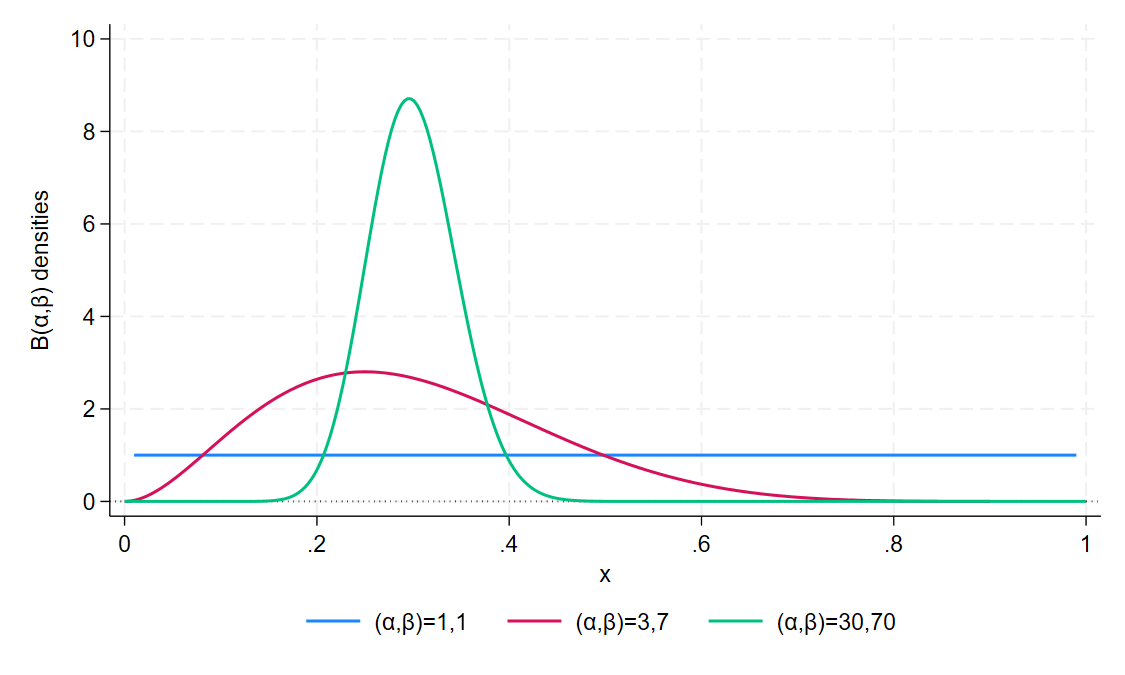
\includegraphics[width=1\textwidth]{figures/3.png}
\end{column}
\end{columns}
\end{frame}

\begin{frame}{Belief Update}
    \begin{itemize}
        \item Prior: $\mathbb{P}(\theta)=\operatorname{Beta}(\theta ; \alpha, \beta) \propto \theta^{\alpha-1}(1-\theta)^{\beta-1}$

\item  Posterior after coin flip:

$$
\begin{aligned}
\mathbb{P}(\theta \mid \text{head}) & \propto \quad\quad\mathbb{P}(\theta) \quad\quad\quad\; \mathbb{P}(\text{head} \mid \theta) \\
& \propto \theta^{\alpha-1}(1-\theta)^{\beta-1} \quad\quad\quad \theta \\
& =\theta^{(\alpha+1)-1}(1-\theta)^{\beta-1} \\
& \propto \textcolor{red1}{\operatorname{Beta}(\theta ; \alpha+1, \beta)} \\
\mathbb{P}(\theta \mid \text{tail}) & \propto \quad\quad\mathbb{P}(\theta) \quad\quad\quad\; \mathbb{P}(\text{tail} \mid \theta) \\
& \propto \theta^{\alpha-1}(1-\theta)^{\beta-1} \quad\quad\;(1-\theta) \\
& =\theta^{\alpha-1}(1-\theta)^{(\beta+1)-1} \\
& \propto \textcolor{red1}{\operatorname{Beta}(\theta ; \alpha, \beta+1)}
\end{aligned}
$$ 
    \end{itemize}
\end{frame}




\begin{frame}{Thompson Sampling Algorithm: Bernoulli Rewards}
    


\begin{tcolorbox}[colframe=black, boxrule=1pt, sharp corners]

\textcolor{red1}{ThompsonSampling $(T)$}

$\quad$$V \leftarrow 0$

$\quad$For $t=1$ to $T$

$\quad$$\quad$Sample $R_1(a), \ldots, R_d(a) \sim \mathbb{P}(R(a)) \; \forall a$

$\quad$$\quad$$\hat{R}(a) \leftarrow \frac{1}{d} \sum_{i=1}^d R_i(a)  \; \forall a$

$\quad$$\quad$$a^* \leftarrow \underset{\operatorname{argmax}}{a} \hat{R}(a)$

$\quad$$\quad$Execute $a^*$ and receive $r$

$\quad$$\quad$$V \leftarrow V+r$

$\quad$$\quad$Update $\mathbb{P}\left(R\left(a^*\right)\right)$ based on $r$

Return $V$




\end{tcolorbox}

\end{frame}



\section{Exploration vs Exploitation}
{
\setbeamercolor{background canvas}{bg=BrewerBlue}
\begin{frame}
\centering
\Huge
\textcolor{white}{Exploration vs Exploitation}
\thispagestyle{empty}
\end{frame}
}


%
%\begin{frame}\frametitle{Thompson Sampling}
%\renewcommand{\baselinestretch}{1}
%\begin{itemize}
    %\item $B(R_{a,t}|\alpha_a,\beta_a)$ denotes the density of the beta distribution for random variable $R_t$ with parameters $\alpha_a$ and $\beta_a$
%
    %\item Posterior distribution $P(\theta|R_t)$ is also beta with parameters that can be updated according to a simple rule:
%\begin{align}\label{eq:updating beta}
%(\alpha_a, \beta_a)= \left\{
%\begin{array}{ll}
%(\alpha_a, \beta_a) & \textrm{if chosen arm} \neq a, \\
%(\alpha_a, \beta_a) + (R_t,1-R_t) & \, \textrm{if chosen arm} = a.\nonumber \\
%\end{array}
%\right. 
%\end{align}
%
%\item $\alpha_a$ or $\beta_a$ increases by one with each observed success or failure
    %\item Distribution more concentrated as $\alpha_a+\beta_a$ grows
    %\item Mean $\alpha_a/(\alpha_a + \beta_a)$ and variance $\frac{\alpha_a \beta_a}{(\alpha_a + \beta_a)^2(\alpha_a + \beta_a + 1)}$
%
%\end{itemize}
%
%\end{frame}




\begin{frame}\frametitle{\cite{Thompson1933,Thompson1935} Sampling}

\begin{figure}[h]
\begin{center}
{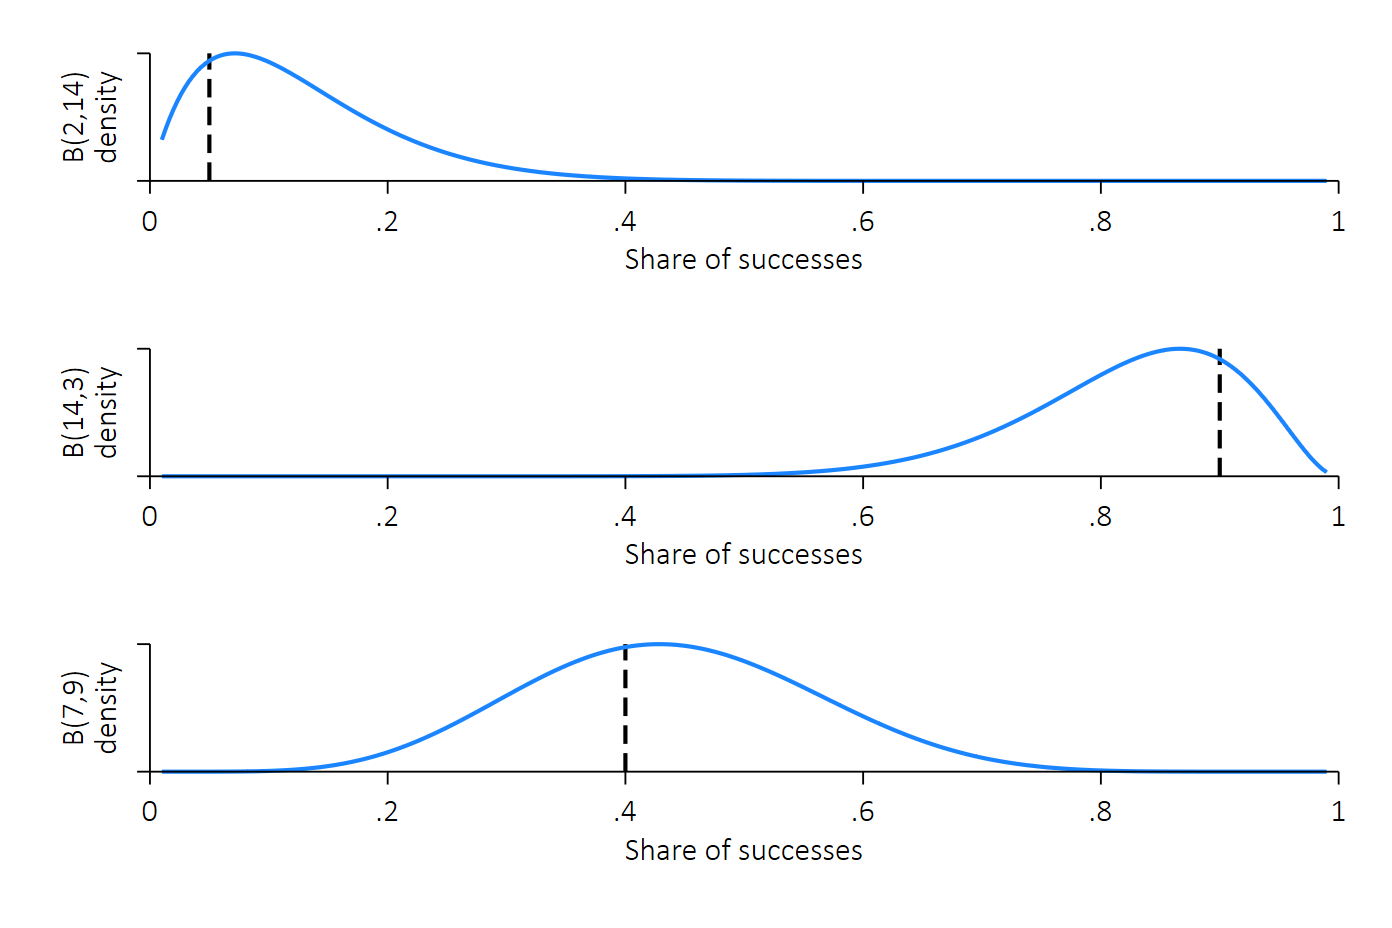
\includegraphics[width=0.9\textwidth]{figures/grafik2.png}}
\end{center}
\vspace*{-4.5ex}
\end{figure}

\begin{itemize}
    \item Beta-Bernoulli Thompson sampling
    \item Models uncertainty about the shape of the distribution and the expected outcome $R$ explicitly\hfill
\small\color{red1}{\href{https://youtu.be/Z8s7oHXEEA4?si=rOTC9CSQTMX7bwBh}{\textbf{Click to watch!}}}

\end{itemize}

\end{frame}



\begin{frame}{Comparison}
\begin{columns}[T]
\begin{column}{0.5\textwidth}
\textbf{Thompson Sampling}
\begin{itemize}
\item   Samples \\
$r_i^a \sim \mathbb{P}\left(r^a ; \theta\right)$
$R_i(a) \sim \mathbb{P}\left(R_i(a) \mid r_1^a \ldots r_t^a\right)$ \\[2ex]

\item   Empirical mean
$
\hat{R}(a)=\frac{1}{d} \sum_{i=1}^d R_i(a)
$\\[2ex]

    
\item   Action Selection
$
a^*=\underset{a}{\operatorname{argmax}}\ \hat{R}(a)
$\\[2ex]

%\item  Observe $r_i$ and update $\theta$

\item   \textcolor{red1}{Some exploration}

\end{itemize}
\end{column}
\begin{column}{0.5\textwidth}
\textbf{Greedy Strategy}
\begin{itemize}
\item  Samples\\
$r_i^a \sim \mathbb{P}\left(r^a ; \theta\right)$\\[4.4ex]

\item  Empirical mean
$
\tilde{R}(a)=\frac{1}{t} \sum_{i=1}^t r_i^a
$\\[2ex]


\item  Action Selection
$a^* = \underset{a}{\operatorname{argmax}}\ \tilde{R}(a)$\\[2ex]

%\item  Observe $r_n$ and update $\theta$

\item \textcolor{red1}{No exploration}
\end{itemize}
\end{column}
\end{columns}
\vspace{8mm}
\citep{russo2018tutorial}
\end{frame}


\begin{frame}{Sample Size}


    \begin{itemize}
        \item In Thompson sampling, amount of data $t$ and sample size $d$ regulate amount of exploration

\item  As $t$ and $d$ increase, $\hat{R}(a)$ becomes less stochastic, which reduces exploration

\begin{itemize}
    
\item  \textcolor{red1}{As $t \uparrow, \mathbb{P}\left(R(a) \mid r_{1}^{a}, \ldots, r_{t}^{a}\right)$ becomes more peaked}
\item  \textcolor{red1}{As $d \uparrow, \hat{R}(a)$ approaches $\mathbb{E}\left[R(a) \mid r_{1}^{a}, \ldots, r_{t}^{a}\right]$}
 
\end{itemize}
\item  The stochasticity of $\hat{R}(a)$ ensures that all actions are chosen with some probability 
    \end{itemize}
\end{frame}

\begin{frame}{Analysis}


\begin{itemize}
    \item Thompson sampling converges to best arm
    \item Theory:
 
\begin{itemize}
    \item Expected cumulative regret: \textcolor{red1}{$\mathcal{O}(\log T)$}
\item On par with UCB and $\varepsilon$-greedy
 
\end{itemize} 
\item Practice:
 \begin{itemize}
     \item Sample size $d$ often set to 1
 
 \end{itemize}
\end{itemize}
    
\end{frame}


\begin{frame}[t,allowframebreaks
]%\nocite{*}
\frametitle{References}
\small
\bibliography{bib}
\end{frame}

\section{Takeaways}
{
\setbeamercolor{background canvas}{bg=BrewerBlue}
\begin{frame}
\centering
\Huge
\textcolor{white}{Takeaways}
\thispagestyle{empty}
\end{frame}
}

\begin{frame}{What is Thompson Sampling?}

\begin{itemize}
    \item Models uncertainty about expected rewards using probability distributions
    \item Samples from posterior of each arm’s reward distribution
		\item Selects the arm with the highest sampled value
    \item Posterior is updated after each observation
    \item Achieves log regret
		\item Applied at, e.g., Google, Amazon, Facebook, Salesforce, and Netflix \pause
		\citep[e.g.,][]{Hill_2017,Scott2015,Agarwal2014,Chapelle2011,Scott2010,Graepel2010}
\end{itemize}
\end{frame}


\end{document}
